\chapter{Steady-state dynamics of the audience applause}
\label{chap3}
\def\statepsi{\mid \psi \; \rangle}
\def\energy{\mid E_{\vec{k}} \; \rangle}
\def\psixt{\mid \psi(x,t) \; \rangle}
\def\statepsixtrev{\mid \psi(x,t=T_{rev}) \; \rangle}
\def\statepsixt0{\mid \psi(x,t=0) \; \rangle}
\def\lowering{S^-_l \mid 0 \; \rangle}
\def\loweringa{S^-_m \; S^-_l \mid 0 \; \rangle}



\section{Steady-state equation for different cases}

\hspace{\parindent} The steady-state conditions are when the state $\vec{n}$ is fixed and when the forcing function expires ($d\vec{n}/dt = 0$ and $f=0$)
Once these conditions are achieved, \eqref{eq:diff1} and \eqref{eq:diff2} are simplified to the steady-state equation for $n_c$:

\begin{equation}\label{eq:steadystate}
\bar{a}(N-n_{c})(N-1 + \beta n_{c}) = b(N-1)^{2}
\end{equation}

where $\bar{a}\equiv a\alpha$. 
The values of steady state $n_{c}$ provided by this equation does not include the trivial solution $n_{c}=0$.
Figure~\ref{fig:system}(b) shows the possible steady-states $n_{c}$ for different $\beta$ values and for $b = 0.5$.
Since $n_{c}>0$, all curves below the $n_{c}=0$ axis are extraneous.
A similar pattern is observed for other values of $b$ where all non-zero curves intersect the $n_{c}=0$ line at around $\bar{a} = b$.

\subsection{Case 1}
Setting $n_{c} = 0$ in \eqref{eq:steadystate} gives us the critical $\bar{a} = \bar{a}_{1}$:

\begin{equation}
\bar{a}_{1} = \frac{b(N-1)}{N}
\end{equation}

which for $N\gg1$ results to the expected $\bar{a}_{1}\approx b$.

The non-trivial solution \eqref{eq:steadystate} is quadratic, with $n_{c}$ resulting to two solutions for a given $\bar{a}$-value and parameters $b$ and $\beta$.
For $\beta\leq1$, the steady-state solutions for $n_{c}>0$ appear uniquely for $\bar{a}>\bar{a}_{1}$.
However, when $\beta>1$, two non-trivial solutions for which $n_{c}>0$ appear between a new critical value of $\bar{a}=\bar{a}_{2}$, corresponding to the vertex of \eqref{eq:steadystate}, and $\bar{a}_{1}$.
This $\bar{a}_{2}$ is given by

\begin{equation}
\bar{a}_{2} = \frac{b(N-1)^{2}}{(N-n_{c}^{*})(N-1+\beta n_{c}^{*})}
\end{equation}

where $n_{c}^{*} \equiv [1+(\beta-1)N]/2\beta$.
This non-trivial solution however, is unstable upon substitution with $\ddot{\vec{n}}$ resulting to $\ddot{\vec{n}}<0$.
Thus, the middle branch in the range $\bar{a}\in(\bar{a}_{2},\bar{a}_{1})$ is an unstable steady-state.
%For $\bar{a} \geq b$, $n_{c}$ has three solutions: the trivial solution $n_{c}=0$ and the two solutions provided by \eqref{eq:steadystate}.
%For certain $\bar{a} < b$ values, a second, non-trivial solution appears.

\section{Phase space for varying parameters}
\hspace{\parindent} By parametrizing the steady-state functions as functions of time, $t$, we can plot the steady-state population, $nC$, versus $\bar{a}$. 
This phase space gives us the steady-state value for any given $\bar{a}$, $b$, and $\beta$. 
For the graphs shown, $b$ is typically constant, and can be identified in the title, while $\beta$ is varied, shown by the various colored curves. 
Both trivial and non-trivial steady-state solutions are shown in the graph. In order to determine which steady-state solution is correct, simulations are performed and their results plotted against the curves. 
 
\section{Simulation experiments}
\hspace{\parindent} We confirm our analytical results by simulating the processes $\mathrm{R}_{1}$ and $\mathrm{R}_{2}$ via an agent-based Monte Carlo method.
For each iteration, each agent is assigned a random number which is then compared to one of the transition probabilities:
\begin{eqnarray}
P(\mathrm{R}_{1}) &=& a(f+f'-f'f)\label{eq:probr1} \\ %REVISION%
P(\mathrm{R}_{2}) &=& bg'\label{eq:probr2}
\end{eqnarray}
Agents at state S transition to state C via $\mathrm{R}_1$ with probability \eqref{eq:probr1} and those at state C transition to state S via $\mathrm{R}_2$ with probability  \eqref{eq:probr2}
%Agents with state S are compared to \eqref{eq:probr1} while those with state C are compared to \eqref{eq:probr2}. 
Monte Carlo procedure 
%for each probabilistic transition 
is done by drawing a uniform random number $u \in [0,1]$ from a random number generator and comparing it with the corresponding probability $P$.
If $u\leq P$ the chosen transition is allowed to occur.

Figure~\ref{fig:parametric}(a) and \ref{fig:parametric}(b) show sample simulations given specific parameters that settle to a certain $n_{c}$ as the simulation time $t$ progresses.
Since the values settles around some value of $n_{c}$ beyond $t>50$~iterations for this value of $N$, we can safely assume that the $n_{c}$ for $t = 100$ is equivalent to $n_{c}$ for $t \rightarrow \infty$.
We took $10$ sample runs with different initial random number generator states and recorded the final $n_{c}$ value for each iteration.
The mean and standard deviation of the steady-state values are then computed for each parameter space $(\bar{a},b,\beta)$.
%This was done for varying $\bar{a}$ and $b$ values at specific $\beta$ values. 
The data points were then plotted with the corresponding parametrized differential curve shown in Fig.~\ref{fig:parametric}(c). 
For $\beta \leq 1$, the simulation is consistent with the trivial steady state solution until it reaches the critical point $b=\bar{a}$, after which follows non-trivial, non-extraneous solution consistent with \eqref{eq:steadystate}.
For $\beta > 1$, the simulation follows the trivial steady-state and then breaks away and approaches the vertex of \eqref{eq:steadystate} at $\bar{a}_{2}$, after which, continues to follow the upper branch of \eqref{eq:steadystate}.    

\subsection{Confirmation of model by simulation}
Shown are the results of the simulation experiments plotted against the steady-state solutions. For all cases, the simulation initially follows the trivial solution until it reaches a certain point and bifurcates to the non-trivial point. For $\beta < 1$ the point of bifurcation is the critical point $\bar{a}$. For $\beta > 1$, the point of bifurcation is an unknown point before $\bar{a}_{2}$, the vertex of the curve. The simulations jump from the trivial solution to points unpredictable by the analytics and then arrive somewhere near the vertex at $\bar{a}_{2}$. After arriving at the critical point, the simulations then follow the upper branch of the non-trivial solution curve. At this point, the lower branch of the non-trivial solution is unknown and will be further investigated. 


\subsection{Unstable points}
For the previous simulation experiments, all agents start at state S and then forced to transition to state C. To investigate the properties of the lower branch on the non-trivial solution, we vary the number of agents that start the simulation in state C and remove the forcing function. This allows us to determine where the system will settle given the specific starting $nC$ value, more particularly for $nC$ values near the lower branch of the non-trivial solution. Shown are the new phase space graphs that include arrows that point to where that $nC$ value for the given $\bar{a}$ settles.
The color of the arrows represents the probability of going towards that direction.
Intuitively for $\beta < 1$, all $nC$ values point towards the trivial solution for all $\bar{a}$ values less than  $\bar{a}_{1}$. 
All $nC$ with $\bar{a}$ values greater than $\bar{a}_{1}$ point towards the non-trival solution.
For $\beta > 1$, what differs is the behavior at the vertex and the lower branch of the non-trivial solution.
$nC$ values above the vertex have an estimated 50\% to either settle at the vertex or zero, while $nC$ values below the vertex absolutely settle to zero.
Points slightly above the lower branch tend more towards settling to the upper branch but still have a chance to settle at 0.
Likewise for points below the lower branch.
Points within the lower branch have a 50\% of settling to either trivial or non trivial solution.



%%

%\begin{figure}[htb]
%\centering
%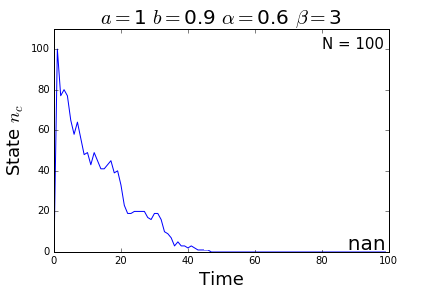
\includegraphics[width=0.3\columnwidth]{simulation/sim1}
%\includegraphics[width=0.3\columnwidth]{simulation/sim2}
%\includegraphics[width=0.6\columnwidth]{sim2}
%\caption{
%Sample simulations for $N = 100$ with the parameters: (a) $\bar{a} = 0.6$, $b = 0.9$ and $\beta = 3$ and (b) $\bar{a} = 0.36$, $b=0.7$ and $\beta = 14$.
%The simulation in (a) settles to the trivial steady-state ($n_{c}=0$) while the results in (b) show an average of $\langle{n_{c}}\rangle\approx85.5\pm 9.53$.
%[!! Remove the labels ``Steady State: ...''. One does not report an average with too many significant digits. What is the actual standard deviation (SD) here? Keep the decimal digits of the reported SD to two maximum.]
%(c) The average of the simulated steady-state values for different parameters are shown together with the theoretical predictions.
%The error bars provide the extent of the sample standard deviations computed. The cross indicates the vertex given by (9), i.e., $\bar{a_{2}}$
%} \label{fig:parametric}
%\end{figure}








